% !TeX root = thesis_main.tex
% ---------------------------------------------------
% ----- Main document of the template
% ----- for Bachelor-, Master thesis and class papers
% ---------------------------------------------------
%  Created by C. Müller-Birn on 2012-08-17, CC-BY-SA 3.0.
%  Last upadte: C. Müller-Birn 2015-11-27
%  Freie Universität Berlin, Institute of Computer Science, Human Centered Computing. 

\documentclass[pdftex,a4paper,12pt,DIV=calc,BCOR5mm,ngerman,twoside,smallheadings,titlepage]{scrbook}   
% ----- weitere Optionen 
%draft,			% Entwurfsmodus zum Anzeigen zu leerer/voller Boxen 
%DIV=calc
%DIV12,			% Seitengröße (siehe Koma Skript Dokumentation !) 
%BCOR5mm,		% Zusätzlicher Rand auf der Innenseite 
%twoside,		% Seitenränder werden an doppelseitig angepasst 
%fleqn,			% Formeln werden linksbündig (und nicht zentriert) angezeigt 
%titlepage,		% Titel wird in einer 'titlepage' Umgebung gesetzt 
%bigheadings,	% Große Überschriften (normal, small-headings) 
%halfparskip-	% Absatz wird nicht eingerückt, dafür aber um eine halbe Zeile nach unten gerückt
%
%---------------------------------------------------
%----- Packages
%---------------------------------------------------
%
\usepackage[T1]{fontenc} 
\usepackage[utf8]{inputenc}
\usepackage[english]{babel} %\usepackage[english]{babel}  
\usepackage{ae} 
\usepackage{bibgerm}    

\usepackage{fancyhdr} % Define simple headings 
\usepackage{xcolor}
\usepackage{url}
\usepackage{listings}
%\usepackage{vmargin} % Adjust margins in a simple way
%
\usepackage{amsmath}
%
\usepackage[pdftex]{graphicx}  
\usepackage{hyperref} % turn all your internal references into hyperlinks
%\usepackage[pdfstartview=FitH,pdftitle={<<Titel der Arbeit>>}, pdfauthor={<<Autor>>}, pdfkeywords={<<Schlüsselwörter>>}, pdfsubject={<<Titel der Arbeit>>}, colorlinks=true, linkcolor=black, citecolor=black, urlcolor=black, hypertexnames=false, bookmarksnumbered=true, bookmarksopen=true, pdfborder = {0 0 0}]{hyperref}
%
% table settings 
\usepackage{booktabs}  
\usepackage{tabularx}  
\usepackage{rotating}
\usepackage{longtable}
\usepackage{pdflscape}
\usepackage{multirow} %multi row
\usepackage{rotating} %for rotating table
%
%---------------------------------------------------
%----- PDF and document setup
%---------------------------------------------------
%
\hypersetup{
	pdftitle={How does an editor for dynamic resources for users with different levels of expertise look like and how can it be conceptualized and implemented within the constraints of an exisiting ecosystem?},  % please, add the title of your thesis
    pdfauthor={Matthias Kind},   % please, add your name
    pdfsubject={Bachelor thesis, Institute of Computer Science, Freie Universität Berlin>}, % please, select the type of this document
    pdfstartview={FitH},    % fits the width of the page to the window
    pdfnewwindow=true, 		% links in new window
    colorlinks=false,  		% false: boxed links; true: colored links
    linkcolor=red,          % color of internal links
    citecolor=green,        % color of links to bibliography
    filecolor=magenta,      % color of file links
    urlcolor=cyan           % color of external links
}
% 
%---------------------------------------------------
%----- Customize page size
%---------------------------------------------------
\usepackage[top=3cm,right=3cm,bottom=4cm,left=4cm]{geometry}    
%
%---------------------------------------------------
%----- Customize header and footer\pagestyle{fancy} 
%---------------------------------------------------
\pagestyle{fancy}

\fancyhf{}  % delete all existing header formating

\fancyhead[LE]{\leftmark}  % represent the current chapter heading in uppercase
\renewcommand{\chaptermark}[1]{ % adapt the shown chapter name: show it in lower case and with chapter number 
\markboth{\thechapter.\ #1}{}}   

\fancyhead[RO]{\rightmark}   % % represent the current section heading in uppercase 
\renewcommand{\sectionmark}[1]{% adapt the shown section name: show it in lower case and with section number 
\markboth{\thesection.\ #1}{}}

\renewcommand{\headrulewidth}{0pt} % remove lines from header
\renewcommand{\footrulewidth}{0pt} % remove lines from header

\fancyfoot{} % delete all existing footer formating
\fancyfoot[LE,RO]{\thepage} % put page number on the left on even page and right on odd page
%
%---------------------------------------------------      
%----- Settings for word separation  
%---------------------------------------------------      
% Help for separation (from package babel, section 22)):
% In german package the following hints are additionally available:
% "- = an explicit hyphen sign, allowing hyphenation in the rest of the word
% "| = disable ligature at this position. (e.g., Schaf"|fell)
% "~ = for a compound word mark without a breakpoint (e.g., bergauf und "~ab)
% "= = for a compound word mark with a breakpoint, allowing hyphenation in the composing words
% "" = like "-, but producing no hyphen sign (e.g., und/""oder)
%
% Describe separation hints here:
\hyphenation{
% Pro-to-koll-in-stan-zen
% Ma-na-ge-ment  Netz-werk-ele-men-ten
% Netz-werk Netz-werk-re-ser-vie-rung
% Netz-werk-adap-ter Fein-ju-stier-ung
% Da-ten-strom-spe-zi-fi-ka-tion Pa-ket-rumpf
% Kon-troll-in-stanz
}
%
%---------------------------------------------------
%----- Restricting including files   
%---------------------------------------------------
% Only files listed here will be included in the PDF document!
% In order to only partially translate the document, for example for bug-fixing, 
% it might be useful to comment out some of the documents.
\includeonly{
title,
declaration,
abstract_en,
abstract_de,
preface,
introduction,
chapters,
conclusion,
appendix
}

%%%%%%%%%%%%%%%%%%%%%%%%%%%%%%%%%%%%%%%%%%%%%%%%%%%%%%
% The content part of the documentent starts here! %%
%%%%%%%%%%%%%%%%%%%%%%%%%%%%%%%%%%%%%%%%%%%%%%%%%%%%%%

\begin{document}
%---------------------------------------------------
%----- Listing and color definition   
%---------------------------------------------------
\definecolor{red}{rgb}{.8,.1,.2}
\definecolor{blue}{rgb}{.2,.3,.7}
\definecolor{lightyellow}{rgb}{1.,1.,.97}
\definecolor{gray}{rgb}{.7,.7,.7}
\definecolor{darkgreen}{rgb}{0,.5,.1}
\definecolor{darkyellow}{rgb}{1.,.7,.3}
\lstloadlanguages{C++,[Objective]C}
\lstset{
		escapeinside={§§}{§§},
        basicstyle=\ttfamily\footnotesize\mdseries,
        columns=fullflexible,% typewriter font look better with fullflex
        keywordstyle=\bfseries\color{blue},
%		identifierstyle=\bfseries,
        commentstyle=\color{darkgreen},      
        stringstyle=\color{red},
        numbers=left,
        numberstyle=\ttfamily\scriptsize\color{gray},
%       stepnumber=5,
%       numberfirstline=true,
        breaklines=true,
%		prebreak=\\,
        showstringspaces=true,
        tabsize=4,
        captionpos=b,
%		framexrightmargin=-.2\textwidth,
        float=htb,
		frame=tb,
		frameshape={RYR}{n}{n}{RYR},
		rulecolor=\color{darkyellow},
        xleftmargin=15pt,
        xrightmargin=4pt,
        aboveskip=\bigskipamount,
        belowskip=\bigskipamount,
		backgroundcolor=\color{lightyellow},
		extendedchars=true,
       	belowcaptionskip=15pt
}

%---------------------------------------------------
%----- Title and declaration   
%---------------------------------------------------
\pagenumbering{alph} % even though, these page numbers are not visible there are necessary to have unique page numbers 
% !TeX root = thesis_main.tex
% ---------------------------------------------------
% ----- Title page of the template
% ----- for Bachelor-, Master thesis and class papers
% ---------------------------------------------------
%  Created by C. Müller-Birn on 2012-08-17, CC-BY-SA 3.0.
%  Freie Universität Berlin, Institute of Computer Science, Human Centered Computing. 
%
\pagestyle{empty}

\begin{titlepage}

\title{
{\small Bachelorarbeit am Institut für Informatik der Freien Universität Berlin}\\
{\small Human-Centered Computing (HCC)}\\
[6ex]
{\LARGE How does an editor for dynamic resources for users with different levels of expertise look like and how can it be conceptualized and implemented within the constraints of an existing ecosystem?}}

% Title laternative ideas:
% Building an Editor for Dynamic Resources: Challenges and Opportunities in an Existing Ecosystem
% Creating an Editor for Dynamic Resources within Constraints: A Case Study

\author{
{\emph{\normalsize{Matthias Kind}}}\\
{\normalsize Matrikelnummer: 5338650}\\
{\normalsize matthias.kind@fu-berlin.de}\\ 
[18ex]   
{\normalsize Betreuer: Florian Berger} \\
{\normalsize Erstgutachterin: Prof. Dr. Claudia Müller-Birn} \\
{\normalsize Zweitgutachter: Prof. Dr. Lutz Prechelt}}
\vspace{6ex}
\date{\normalsize Berlin, 30.1.2023}
\maketitle
\end{titlepage}

% ---------------------------------------------------
% ----- Declaration of the template
% ----- for Bachelor-, Master thesis and class papers
% ---------------------------------------------------
%  Created by C. Müller-Birn on 2012-08-17, CC-BY-SA 3.0.
%  Freie Universität Berlin, Institute of Computer Science, Human Centered Computing. 
%
\pagestyle{empty}

\subsection*{Eidesstattliche Erklärung}

Ich versichere hiermit an Eides Statt, dass diese Arbeit von niemand anderem als meiner Person verfasst worden ist. Alle verwendeten Hilfsmittel wie Berichte, Bücher, Internetseiten oder ähnliches sind im Literaturverzeichnis angegeben, Zitate aus fremden Arbeiten sind als solche kenntlich gemacht. Die Arbeit wurde bisher in gleicher oder ähnlicher Form keiner anderen Prüfungskommission vorgelegt und auch nicht veröffentlicht.
\par\bigskip  
\noindent Berlin, den \today

\vspace{1.2cm}

\noindent Matthias Kind

\cleardoublepage

%---------------------------------------------------
%----- Abstracts in English and German   
%---------------------------------------------------

% !TeX root = thesis_main.tex
% ---------------------------------------------------
% ----- Abstract (English) of the template
% ----- for Bachelor-, Master thesis and class papers
% ---------------------------------------------------
%  Created by C. Müller-Birn on 2012-08-17, CC-BY-SA 3.0.
%  Freie Universität Berlin, Institute of Computer Science, Human Centered Computing. 
%
\pagestyle{empty}

\subsection*{Abstract}

With the shift from print to digital publishing in the magazine and news publisher world in recent years, the needs to quickly build apps and websites and have them configured as easy as possible gained importance.
While companies already progressed in that field with website builders, headless content management systems and more, internal tools and software used by the administrators of the publishing houses also need to evolve and improve over time, as expectations requirements change.
\\\\
The goal if this bachelor thesis is to conceptualize, plan and implement an UI Editor for the mentioned kinds of apps / websites, written inside an company providing a ''digital publishing suite'' to publishers mainly in Germany and the UK.
There, a web framework (called ''Purple Experience'') is used to deliver apps and websites generated from the same configuration and assets to the end users. This service is closely linked to other existing software systems to edit the contents, manage apps and content delivery and more.
\\
This brownfield project provides some special burdens as well as opportunities,
as the flexibility is restricted by exisitng workflows and software, but also a diverse group existing users with different levels of experience with those software products.
They consist of internal framework developers, customer support, project develoeprs or external people at the publishing houses.
These possible future users of the software created for this thesis provided valuable insights
into their current workflows and how they imagine this tool could improve their productivity and be more enjoable to use.
\\
To gain these insights, I evaulated the use and then applied multiple user research methods like moderated observations, interviews and small questionaires.
Due to the limited size of the user group, the goal was not to gain <TODO> with high diversity of their demographics, but to have information saturation from fewer but more valuable insights into peolpe with diffrent workflows.
\\
The outcome should be usable as guidance for future software development projects for internal tools at companies or environments where the product is limited in it's flexibility but should still give the best user experience possible.
\\\\
Based on the evaulations oth the user research phase, I built an interactive prototype using modern web technologies like react, express.js and Typescript.
This was deployed using continous integration to a controlled group of test users. This allowed to get quick feedback and iterate fast, until the tool can be made available to a broader audience.
\\\\
TODO: the outcomes of the thesis consist of a working software product that is actively used by early adopters, as well 

\cleardoublepage

% ---------------------------------------------------
% ----- Abstract (German) of the template
% ----- for Bachelor-, Master thesis and class papers
% ---------------------------------------------------
%  Created by C. Müller-Birn on 2012-08-17, CC-BY-SA 3.0.
%  Freie Universität Berlin, Institute of Computer Science, Human Centered Computing. 
%
% \pagestyle{empty}

\chapter{Zusammenfassung}

<Hier sollten Sie eine kurze, aussagekräftige Zusammenfassung (ca. eine Seite) Ihrer Arbeit geben, welche das Thema der Arbeit, die wichtigsten Inhalte, die Arbeitsergebnisse und die Bewertung der Ergebnisse umfasst.> 
  
                                          
%---------------------------------------------------
%----- Directories   
%---------------------------------------------------

\frontmatter 
\pagenumbering{roman}

\tableofcontents
\setcounter{tocdepth}{3}   % reduce the included sections in the table of content

\listoffigures
\listoftables

%---------------------------------------------------
%----- Main part
%---------------------------------------------------
\mainmatter
\pagenumbering{arabic} 
\pagestyle{fancy} 

% ---------------------------------------------------
% ----- Preface of the template
% ----- for Bachelor-, Master thesis and class papers
% ---------------------------------------------------
%  Created by C. Müller-Birn on 2012-08-17, CC-BY-SA 3.0.
%  Freie Universität Berlin, Institute of Computer Science, Human Centered Computing. 
%
\chapter*{Vorwort}
\label{chap:preface}

\section*{Allgemeine Hinweise zur Erstellung einer Abschlussarbeit}

\begin{itemize}
	\item Beachten Sie, dass diese Vorlage für einen zweiseitigen Ausdruck angelegt wurde.  
	\item Über die Papierqualität können Sie entscheiden, aber wir empfehlen aber Seiten mit wichtigen, farbigen Grafiken auch in Farbe auszudrucken und dabei ein höherwertiges Papier zu verwenden. 
	\item Bitte stimmen Sie mit dem Betreuer Ihrer Arbeit auch den Zweitgutachter ab. Die Anfrage des Zweitgutachters erfolgt von Ihnen. Es ist an dieser Stelle sinnvoll, die Anfrage mit einer kurzen Zusammenfassung der Arbeit zu stellen.  
	\item Bitte beachten Sie, dass Sie Ihre Abschlussarbeit mit einer Klebebindung versehen, eine Ringbindung ist nicht erwünscht. 
\end{itemize} 

% !TeX root = thesis_main.tex
% ---------------------------------------------------
% ----- Introduction of the template
% ----- for Bachelor-, Master thesis and class papers
% ---------------------------------------------------
%  Created by C. Müller-Birn on 2012-08-17, CC-BY-SA 3.0.
%  Last upadte: C. Müller-Birn 2015-11-27 
%  Freie Universität Berlin, Institute of Computer Science, Human Centered Computing. 
%
\chapter{Introduction}
\label{chap:introduction}

\section{Topic and context}

In the ever-growing world of software development, many companies are now in the situation to maintain a large software ecosystem with complex dependencies.
Still, there is need for continuous improvement and development to stay competitive.
% but still want to improve their systems by developing new components and tools.
This poses the challenge of improving the software from aspects like user experience, scalability and maintainability while being restricted by the ecosystem.
\\
From my point of view, \Gls{greenfield} seems to be implicitly assumed in many books and articles about HCI.
This assumption is not applicable to the situation many software companies are in today.
\\
In a \Gls{brownfield} project, HCI methods need to be adapted to account for technical constraints while still addressing user needs.
User research in general is often neglected due to tight deadlines and limited resources which usually leads to premature releases and unstable software.
This thesis therefore aims to demonstrate the advantages of structured user research in theory as well as in practice, using the case study "UI Editor".

\section{Goals of this thesis}
The goal is to demonstrate how HCI principles and methods can be applied in a brownfield project, using a real-world case study at the company Sprylab as an example.
Sprylab is a company which is engaged in the digital publishing industry, providing Software-as-a-Service (\Gls{saas}) to publishing houses for editing and distributing content.
% Intro UI Editor
The case study consists of the redevelopment of a UI Editor to improve user experience and usability for web developers, admins and editors.

\newpage
\section{Process for research, prototyping and implementation}

The software design process used to develop the UI Editor is described in \cite[p. 104]{LearnHCI:2020ys}.
There, the process is divided into the three phases ``\Gls{design-thinking}'', ``\Gls{lean-ux}'' and ``\Gls{agile}'' (for more details see Glossary).

For this concrete case study, the process looks like this:
\begin{figure}[h]
  \centering
  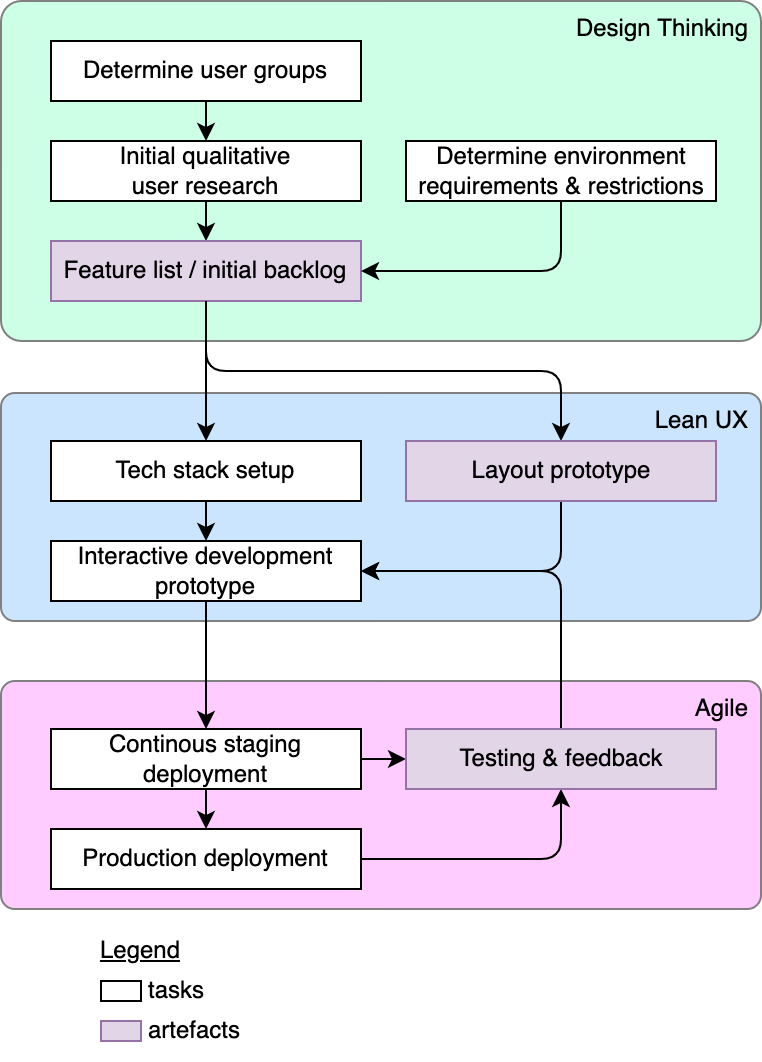
\includegraphics[width=0.8\linewidth]{pics/process.drawio.png}
  \caption{Software design process for the UI Editor.}
	\label{fig:process}
\end{figure}


% !TeX root = ../thesis_main.tex
% ---------------------------------------------------
% ----- Chapters of the template
% ----- for Bachelor-, Master thesis and class papers
% ---------------------------------------------------
%  Created by C. Müller-Birn on 2012-08-17, CC-BY-SA 3.0.
%  Freie Universität Berlin, Institute of Computer Science, Human Centered Computing. 
%
\chapter{Kapitel}
\label{chap:chapters} 

\begin{itemize}
	\item Abhängig vom Ziel der Arbeit und dem verwendeten Forschungsdesign unterscheidet sich dieser Hauptteil der Arbeit erheblich. 
	\item Eine sehr allgemeine Struktur ist die folgende:
	\begin{itemize}
		\item Hintergrund der Arbeit (Theoretische Einordnung der Arbeit) 
		 	\begin{itemize}
		 		\item Hier sollte enthalten sein, welche Anwendungen in diesem Bereich bereits existieren und warum bei diesen ein Defizit besteht. 
				\item Falls genutzt, sollten hier die entsprechenden Algorithmen erläutert werden.
				\item Es sollten die Ziele der Anwendungsentwicklung, d.h. die Anforderungen herausgearbeitet werden. Dabei sollte die bestehende Literatur geeignet integriert werden.
		 	\end{itemize}
		\item Umsetzung (Praktischer Anteil der Arbeit)
			\begin{itemize}
				\item Zunächst sollte die Softwarearchitektur und die genutzten Anwendungen, APIs etc. erläutert werden. Ebenfalls gehört dazu das Datenbankschema.
				\item Es sollten die zentralen Elemente der Software (abhängig von der Aufgabenstellung) beschrieben werden, wie implementierte Algorithmen oder das Oberflächendesign.
				\item Zentraler Quellcode sollte entsprechend aufgelistet werden:
				\lstset{language=Java,basicstyle=\footnotesize,numbers=left,showstringspaces=false,frame=single}
				\begin{lstlisting}
				public class Main {
					public static void main(String[] args) {
						System.out.println("Hello World!");
					}
				}
				\end{lstlisting} 
				%\item Klassendiagramm für Backend
				%\item Dr Quellcode zentraler Implementierungen  können als Auszug in den Anhang. Im Text kann dann darauf verwiesen werden.
			\end{itemize}
		\item Evaluation (zumeist nur für Masterarbeiten relevant)
		\begin{itemize}
			\item Jede Software muss auch getestet werden. Dieses Tests werden entweder mit einem vorgegebenen Datensatz erfolgen oder aber die Evaluation erfolgt auf Basis von Experimenten. In diesem Kapitel sollte daher entweder der genutzte Datensatz oder der experimentelle Aufbau beschrieben werden. 
		\end{itemize}
		\item Ergebnis und Diskussion
		\begin{itemize}
			\item Die Ergebnisse der Anwendung werden in diesem Kapitel vorgestellt und anschließend diskutiert. Wenn möglich sollte die Ergebnisse in Relation zu bestehenden Arbeiten in dem Bereich erörtert werden.
		\end{itemize}
	\end{itemize}  
\end{itemize}
% ---------------------------------------------------
% ----- Conclusion of the template
% ----- for Bachelor-, Master thesis and class papers
% ---------------------------------------------------
%  Created by C. Müller-Birn on 2012-08-17, CC-BY-SA 3.0.
%  Freie Universität Berlin, Institute of Computer Science, Human Centered Computing. 
%
\chapter{Conclusion and outlook}
\label{chap:conclusion}      
This thesis demonstrates the challenges and opportunities of applying HCI principles and methods in a brownfield software development project through the redevelopment of a UI Editor for a digital publishing company, Sprylab.
During the process, it was shown how common user research methods can be adapted to this specific case study and how technical limits and needs of users can be combined in this context.
Agile development and Lean UX enabled iterating quickly and achieving fast deployments to a staging system.
A growing group of users at Sprylab already uses the software in production.
\\\\
The consistently positive feedback shows that the chosen methods and features derived from their outcome were the right approach to enhance the user experience while complying with constraints imposed by the ecosystem.
Also, the way users were involved during the whole process led to a high level of acceptance and interest in supporting the project.
Additionally, this thesis can help to argue for the use of HCI methods in future projects started at Sprylab as well.
I'm confident that this new software is a stable and extensible tool, especially regarding the two factors Usability and Time-on-Task.
In addition to increasing user satisfaction, it also leads to enhancing productivity and customer satisfaction.

TODO: the editor enables users to safely edit JSON configurations and change assets and styles while directly seeing these changes in a preview frame
\\\\
However, there is still room for improvements in terms of accessibility and entry hurdle for new users.
The entry hurdle is still high and a lot of background knowledge is assumed, which is partly due to the complexity of other systems in the ecosystem that were set as technical requirements from the beginning on.
Moving forward, replacing the JSON editor with a custom implementation that combines JSON Schemata and generated UI is one of the next steps, which will speed up the user's
workflow even more and allow for further improvements that are impossible with a third-party library.
\\\\
Overall, this thesis has demonstrated the importance of considering HCI principles and methods in brownfield software development projects, and the potential benefits that can be achieved when these approaches are applied in a real-world context.


%---------------------------------------------------
%----- Bibliography
%---------------------------------------------------
\phantomsection
\addcontentsline{toc}{chapter}{Literatur}
\bibliographystyle{alpha}
\bibliography{references.bib}


%---------------------------------------------------
%----- Appendix   
%---------------------------------------------------
\backmatter
% ---------------------------------------------------
% ----- Appendix of the template
% ----- for Bachelor-, Master thesis and class papers
% ---------------------------------------------------
%  Created by C. Müller-Birn on 2012-08-17, CC-BY-SA 3.0.
%  Freie Universität Berlin, Institute of Computer Science, Human Centered Computing. 
%

\chapter{Appendix}
\label{ch:Appendix}

\section{Erster Teil Appendix}
\label{app:first_appendix} 

\section{Zweiter Teil Appendix}
\label{app:second_appendix}  



\end{document}